\chapter{Background \& Related Work}
\label{chap:background}

%Nic has read

%\begin{itemize}%
%    \item Previous characterisations of Access Patterns
%        \item Static Content
%        \item Video-on-Demand
%            \item Popularity
%            \item Popularity Over Time / Recommendations
%            \item Session duration
%            \item Interactivity
%            \item Popularity Within Content

%        \item Live Streaming
%				\item Popularity
%				\item Time-of-day
%				\item Session duration
%				\item Interactivity

%    \item Discussion on Interactivity and how it breaks streaming
%        \item Introduction
%        \item Push/Pull Techniques
%        \item Hybrid concepts

%    \item Papers about VoD systems, such as YouTube, and M\$'s
%        \item Delivery techniques
%        \item Caching techniques
%        \item VoD Websites (YouTube, etc)
%        \item Overview
%        \item Describe what's typical on these services
%        \item Describe what problems they have
%

%\end{itemize}

%\item Papers about VoD systems, such as YouTube, and M\$'s
%\begin{itemize}
%    \item Overview
%    \item Describe what's typical on these services
%    \item Describe what problems they have
%\end{itemize}

% YouTube paper (I tube, you tube, everybody tubes: analyzing the world's largest user generated content video system)
% M$ VoD Paper (Can Internet Video-on-Demand Be Profitable?)
% Chinese Telecom paper (

%\todo{Explain the focus of this research, and how interactive apps do exist, but what are their limitations}


The focus of this thesis is understanding how video-on-demand (VoD) systems operate under highly interactive workloads. Once a firm understanding of this is achieved, then new techniques can be designed to help improve performance in such systems. Therefore, the first section of this chapter aims to explain how currently deployed VoD systems work. Special attention is paid to which interactive features these systems already provide, as well as their limitations in providing advanced interactivity. This covers systems such as the incredibly popular YouTube~\cite{youtube}, serving low quality short video clips via a content distribution network (CDN), to systems such as BBC iPlayer~\cite{iplayer}, a hybrid peer-to-peer CDN platform offing high quality professional content.

Later, to understand exactly how workloads are analysed, \autoref{sect:characterisations}, provides a detailed overview of how existing characterisation studies have try to explain and model user behaviour. Modelling behaviour is very important for designing video-on-demand mechanisms, for example, understanding the popularity of objects helps to make caching and replication decisions. Most of the existing research on characterising user behaviour has either ignored, or not experienced high levels of interactivity. This is counter to the results displayed later in this thesis. As such, the review of previous work is discussed in the context of interactive workloads, where applicable. This helps motivate the experiments evaluated in \autoref{chap:evaluation}, as well as providing a solid ground to understand the problems with interactivity.

%Finally, \autoref{sect:deliverinteract} expands on the previous two section by highlighting what related research has gone into creating scalable and efficient systems for providing interactivity. This forms the background knowledge for \autoref{chap:new_techiques}.

\section{Deployed Video-on-Demand Systems}
\label{sect:video-on-demand}
%    The content length is shortened by two orders of magnitude and so is the production time.
%     Wired magazine refers to this small-sized content pop culture as �bite-size bits for high-speed munching� [34].
%    [34] N. Miller. Manifesto for a New Age. Wired Magazine, March 2007

    There are multiple systems now in place, which allow users to watch videos when they want, how they want. There is an abundance of content available, ranging from short funny video clips, to long feature movies, and everything in between. This has been driven by incredible demand, causing new video-on-demand (VoD) systems to appear, almost daily, to serve different niches. To keep up with demands, these videos are no longer just made by professionals. Anyone with a cheap camcorder or webcam can become famous for 5~minutes. Wired magazine refers to this as ``bite-size bits for high-speed munching''~\cite{miller2008mfa}.

    As VoD is becoming more ubiquitous, users are expecting more features. One such feature is interactivity, the ability to pause, resume, and seek within the content. Many of these VoD systems are offering interactive features, however, each with their own limitations. For example, some can only offer interactivity by forcing the user to download the full video first. If they do allow interactivity via streaming, then the systems seem slow or sluggish.

    This section highlights the main classes of VoD applications, and well as how they work. Their interactivity features are discussed in detail, as well as their flaws. At the end of this section, there is a summary of all solutions, giving a quick overview of what is out there, and how it operates.

\subsection{Flash-based Sites}
\label{sect:ugc}
%Checked by Nic

\begin{table}
\center
\begin{tabular}{|rccc|}
\hline
\setrowcolor{TableRowHead}
                                          & YouTube &   Dailymotion  &    Metacafe    \\
\hline
\setrowcolor{TableRowA}
  Unique Visitors ($\times 10^6$/month)   & 70      & 10             & 10             \\
\setrowcolor{TableRowB}
  Videos Watched ($\times 10^6$/day)      & 100     & 25             & 15             \\
\setrowcolor{TableRowA}
  Alexa Site Rank (Feb '08)               & 3       & 31             & 179            \\
\setrowcolor{TableRowB}
  Stored Videos (2006)                    & 45 TB   & \emph{unknown} & \emph{unknown} \\
\setrowcolor{TableRowA}
  Stored Videos (2007)                    & 357 TB  & \emph{unknown} & \emph{unknown} \\
\hline
\end{tabular}
\caption[Overview of the most popular video sharing websites]{Overview of the most popular video sharing websites, adapted from~\cite{saxena2008avs,cheng2007uci}}
\label{tab:videosites}
\end{table}

    A big push in storing videos online has been the creation of \emph{user generated content} (UGC) websites such as YouTube~\cite{youtube}, Dailymotion~\cite{dailymotion}, Metacafe~\cite{metacafe} as well as many more~\cite{msnvideo,googlevideo,hulu,myspacetv}. The most popular of these sites, YouTube, was founded in 2005. Despite only being three years old, it is now the 3\rd most popular site on the internet, illustrating how popular these sites are. \autoref{tab:videosites} gives a brief overview of the most commonly used UGC sites' popularity, as well as how many videos are viewed and stored on these services.

    These Web 2.0\footnote{Web 2.0 is a term to describe a new generation of websites, where the site's value comes from the users who participate.} websites allow users to upload their own videos for others to watch freely. Once uploaded, other users can begin tagging~\cite{ames2007wtm}, rating and commenting on each video. Users may also share their favorite videos with their friends, allowing the video to quickly disseminate through a video sharing social network.

    Typically the content on the sites is short low quality clips. A study of YouTube by Cheng~\emph{et~al.} found that 97.8\% of all videos were shorter than 10 minutes~\cite{cheng2007uci}. This is due to a limit imposed by YouTube, that regular users may only upload videos 10 minutes or shorter. A different study found that the mean viewing length was 4.15~minutes with a median of 3.33~minutes~\cite{gill2007ytc}. There is a small group of authorized users who may upload longer videos, which includes content such as documentaries or lectures. These short length videos are not representative of all sites; an analysis of MSN Video found that many of the videos were a lot longer than YouTube, however no exact figures or distributions of lengths were offered~\cite{huang2007civ}.

    These sites typically use \emph{pseudo-streaming} (or sometimes called \emph{progressive download}) techniques~\cite{guo2005amw}. This is where a media file is downloaded using general file downloading techniques, but as it downloads it is also played. As a true streaming protocol is not used, many features are lacking, for example, the rate the server transmission the file will not be synchronised with the playback rate. This may cause the stream to be received faster or slower than required. Additionally controls such as pause or seeking are not easily available.

    The most common example of \emph{pseudo-streaming} involves a combination of an Adobe Flash player and HTTP downloading. A web page contains a Flash video player which requests a Flash video file (FLV) from the HTTP server. The Flash file is downloaded just like any other file would be via HTTP. As the file downloads, the Flash player can begin playback.

    Flash video was chosen due to its widespread deployment. For example, in 2000, the Flash player was distributed with AOL, Netscape and Internet Explorer browsers. Later, in 2002, the Flash player came pre-installed with Windows XP. This lead to an unverified claim that Flash Player had an install-base of roughly 92\% of all internet users~\cite{wiki_flash}.

    Flash video can be compressed using various encodings. On YouTube, the video is encoded with the Sorenson Spark H.263 codec, with a resolution of 320x240 at 25 frames per second~\cite{cheng2007uci}. This creates videos which have a bitrate of around 330~kbps. However, YouTube is at the lower end of quality, compared to other UGC sites. Due to home broadband becoming more ubiquitous, there has been greater demand for higher quality videos. For example, in February 2008, Dailymotion announced that it would begin streaming at the high-definition resolution of 720p~(1280x720)~\cite{lowensohn2008dgh}, requiring at least 8-16~Mbps bitrate streams.

\begin{figure}[t]
    \centering

    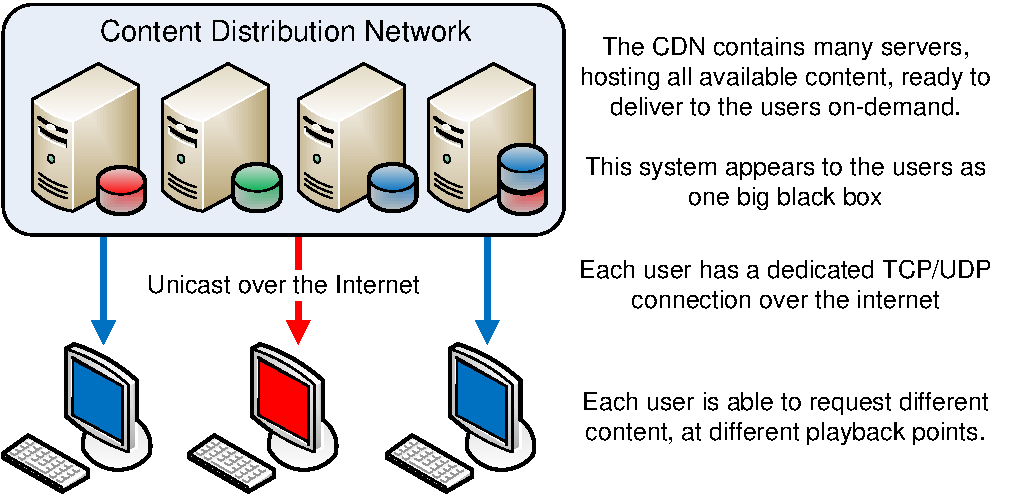
\includegraphics[width=0.7\columnwidth]{./diagrams/CDN}

    \caption
        [Distribution of media via a content distribution network]
        {Distribution of media via a content distribution network. Different coloured arrows and shapes represent the different content.}
    \label{fig:cdn}
\end{figure}

    The HTTP servers used for streaming are typically hosted by a content distribution network (CDN) as depicted in \autoref{fig:cdn}. Little is known about how these systems are configured and deployed, however some research has gone into inferring their deployment by taking measurements. In one study, Saxena~\emph{et~al.} found that YouTube's videos are served from just two main locations in the US; San Mateo (77\%) and Mountain View (22\%), with the remaining 1\% being served by the Limelight's CDN~\cite{saxena2008avs}. This suggests most of YouTube's CDN is built and controlled in-house. Saxena~\emph{et~al.} also found that Metacafe took a different approach and outsourced their needs to the Akamai and L3 Networks CDNs. It is well know that Akamai position their servers into as many ISP's points of presence (POPs) as possible~\cite{huang2008uhc}.

    Until very recently these UGC sites had limited interactive controls. The Flash player would continue to buffer the video being viewed as fast as possible and store everything which has been received in a temporary file on the computer's hard disk. Users were able to pause, and seek backwards into the stored buffer, but were unable to seek ahead of the buffer. Since late 2007/early 2008, YouTube and others have begun allowing arbitrary seeks anywhere in the media before it is buffered. This has been achieved using a custom client-side Flash player and some server software. How exactly this is achieved is discussed later in \autoref{sect:seekable_flash}, as this technique was developed independently by us before it had been implemented by YouTube.

\subsection{BBC iPlayer}
\label{sect:bbciplayer}
% Nic has read
%TODO Last sentence mentions network PVRs before they are discussed!

    BBC iPlayer~\cite{iplayer} has been leading the way as a new type of desktop application which enables users to watch video-on-demand over the internet, using a normal home broadband connection. BSkyB and Channel~4 have also created similar products to compete with the BBC, named Sky Player~\cite{skyplayer} and 4oD~\cite{4od} respectively. These products differ from network PVRs, as they serve a more specific task, and do not require custom hardware.

    These products offer a catalogue of old programmes (which are no longer regularly shown on broadcast TV), and access to most of the broadcast programming shown in the last 7~days. Users can select which programme they want, and their client begins to download the video. However, these products do not stream the video; instead they download a single file. This means the user must wait until the full file is downloaded before playback can start.

    All three applications are actually based on one companies technology, Kontiki~\cite{Kontiki}. This company has created their own technology to provide a content delivery platform, which can securely deliver media from standard servers, assisted by scalable peer-to-peer techniques. Kontiki is closed source software, and as far as we are aware no studies have been conducted to analyse how it works. However, from promotional material, it constructs a simple peer-to-peer network from the users. This network can be configured to limit how the peers are connected, for example, making sure the peers do not connect outside of their own subnet, or autonomous system (AS) boundary.

    When a Kontiki client is idle, any spare bandwidth is used to help spread the content within the network. To seed the content into the peer-to-peer network, and to provide additional capacity, a normal network of servers deployed in a CDN are used. This peer-to-peer network does not allow users to publish their own content, as the network is used just as the provider's content delivery platform. To ensure this requirement is met, the network uses strong cryptographic techniques such as asymmetric cryptography~\cite{rivest1978mfo}, to guarantee that media is not tampered with, and also to ensure that new media is not injected into the network without permission.

    The files published by the BBC are typically Windows Media (WMV) files, protected with digital rights management (DRM). The DRM stops the files from being shared with others, and expires the files a few days after playback. These files are of good quality, and are roughly 140~MB for a 30~minute show. Since the full WMV files are downloaded before playback can begin, interactive controls are easy to provide. Pausing and seeking to arbitrary points is readily available, and instantaneous.

    Due to the Kontiki platform, and the DRM techniques, the iPlayer software only runs on Microsoft Windows, and not on other operating systems such as Linux, or Apple's Mac OS. This received many criticisms, as the publicly funded BBC were ignoring a subset of the public that did not use Windows. To counter, this the BBC introduced a new streaming based iPlayer which could be accessed via their website. This uses Adobe Flash technology, similar to that used by many user generated content sites, such as YouTube. By creating their Flash based site, any device which could render Flash video was now able to view the iPlayer's catalogue. This includes desktop computers running various free operating systems, many home gaming consoles, such as the Nintendo Wii~\cite{bbc2008ban} and Sony Playstation 3~\cite{purchese2008fmb}, and mobile devices such as the Apple iPhone~\cite{bbc2008bic}.

%    \todo{Briefly recap what interactive features are available with the online iPlayer}

\subsection{Personal Video Recorders}
\label{sect:pvr}

% Nic has read

\begin{figure}[t]
    \centering

    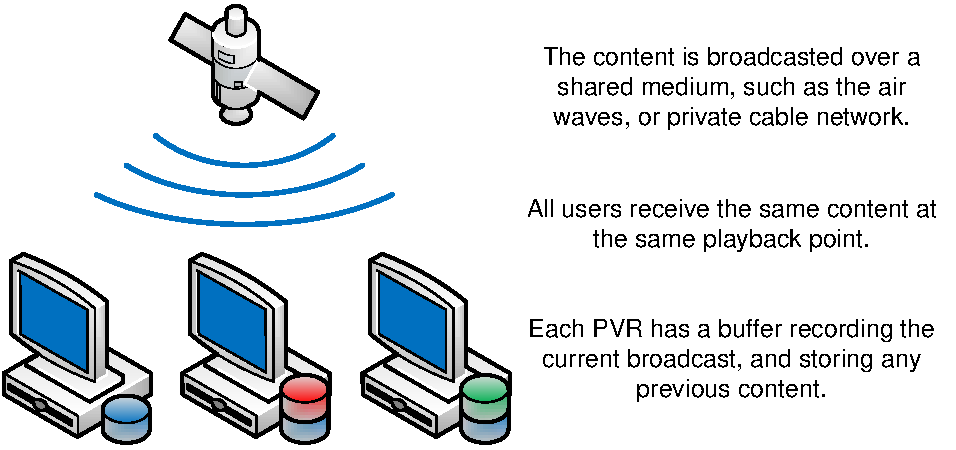
\includegraphics[width=0.7\columnwidth]{./diagrams/PVR}

    \caption
        [Distribution of media in a boardcast personal video recorder network]
        {Distribution of media in a boardcast personal video recorder network. Different coloured arrows and shapes represent the different content.}
    \label{fig:pvr}
\end{figure}

    %"More than half (57\%) of all UK residents �time-shift� their TV viewing, using on-demand TV services or recording live television for viewing later", "36\% use a PVR"~\cite{YouGov2008red}

    A device that is becoming more commonplace in the living room, is the \emph{time-shifting} set-top box. These devices, sometimes called personal video recorder (PVR) or digital video recorder (DVR), are typically set-top boxes which record broadcast TV. These PVRs allow the user to pause playback while the box continues to record, or rewind within the recording. Additionally, if the user has paused or rewound, they may fast forward to catch up with the live broadcast. It was estimated in 2008 that 36\% of the UK uses a PVR~\cite{YouGov2008red}.

    There are many PVRs on the market, the most popular being, Sky+~\cite{sky+}, TiVo~\cite{tivo}, ReplayTV~\cite{replaytv} and UltimateTV~\cite{ultimatetv}. The Sky+ PVR, for example, records broadcast TV received via a satellite dish as seen in \autoref{fig:pvr}. This PVR has two TV tuners, allowing it to record from two channels simultaneously. As with most of these devices, it contains a large hard disk, able to record within the range of 40 to 80~hours of TV.

    The Sky+ box can be scheduled to record future TV programmes or films via the electronic programme guide (EPG). Once recorded, the user is able to play the recorded programmes by selecting them from the EPG. However, this does not give the user a true video-on-demand experience, as they have to wait until the programme airs before being able to watch it. To combat this, Sky+ has recently integrated a \emph{push video-on-demand} system called ``Sky Anytime''. Sky can instruct the Sky+ box to record popular programming, such as new movies, or sporting events. The programming is sent on hidden broadcast channels, typically during the night when the Sky+ box is not in use. Users can then chose any of these ``Anytime'' programmes, and play them back instantly from their local hard disks.

    The interactive controls are rather limited with these boxes, as they are only able to seek within what is currently buffered. In live TV that means rewinding, but in pre-recorded content (such as ``Sky Anytime'') they may fast-forward or rewind. To allow rewinding with live TV, the Sky+ box is always recording the current channel, with a buffer of up to two hours. Once the channel changes, this buffer is discarded and a new one begins. This allows a user to pause for no longer than two hours, and rewind the current channel up to a maximum of two hours (as long as the channel is not changed within that time).

    %TODO cite staggered broadcast
    Most satellite providers also offer pay-per-view content, such as very new movies, or live one-off sporting events. Events, such as sports, are typically broadcast live on a single encrypted channel, which limits the interactivity to simple pause and rewind. More interesting are the \emph{near video-on-demand} services. These are typically provided for movies, where a single movie will be broadcast on multiple channels using a simple staggered broadcast technique. If staggered, the movie will be broadcasted at fixed time intervals, for example, every 15 minutes. Thus, when a user purchases a movie they will have to wait up to 15 minutes to begin watching.

    Near video-on-demand has the ability to allow users to seek forward or backwards in fixed time intervals, for example, 15 minutes at a time. When combined with a PVR, this can be extended to allow more fine grained seeking, if for example, the PVR records two broadcast channels at different positions within one programme. This could allow the PVR to buffer 15 minutes ahead, by using the second channel. Once the first channel has caught up to the buffer, it can begin playback from the buffer, and use the first channel to record 30 minutes ahead. This process can continue until the full movie is buffered to disk. As far as we are aware, no set-top box offers such functionality, mostly due to the added complexity for little gain.

\subsection{Networked Set-top Boxes (IPTV)}
%Nic has read

    %TODO \cite{olausson2007gif} predicts there will be 80 million IPTV users by 2011

    Some set-top boxes, those typically on cable networks, have begun to roll out IPTV services which offer true video-on-demand. In the UK, the main provider is Virgin Media with over 3 million customers using its ``On Demand'' service~\cite{virgin2008on}. British Telecom (BT) have also recently introduced a similar product called ``BT Vision''~\cite{bt2008bv}. It is predicted that by 2011, there will be 80~million IPTV users worldwide~\cite{olausson2007gif}.

    In these systems, a simple set-top box or PVR is connected to either a private network (in the case of Virgin Media), or via the public internet. Content is then streamed directly to the user instantly, on-demand. Virgin Media have been able to offer this service for many years by utilising the existing cable network infrastructure to unicast video from the user's local head-end\footnote{A head-end is a facility run by a cable company to serve customers in the local region}  directly to the end-user. This is not possible in satellite or traditional radio broadcast as both have finite broadcast capacity, whereas cable networks have constantly invested in and improved their networks over the years, adding more and more capacity.

    Nevertheless, the on-demand content which is available via these services seems to be of lower than normal broadcast quality, and little is known about the technical details. However, from experiments with these set-top boxes it may be possible to infer how they operate. For example, examining Virgin Media's On Demand service, it is clear that a staggered broadcast system is being used. When seeking through the video, the video jumps in increments of 15 seconds, and when starting a new video it takes up to 15~seconds to begin. This may be because the video is being broadcast in staggered intervals of 15~seconds. It is unclear if this is done so a broadcast technique such as multicast may be used, or if this is to reduce the number of unique channels the server has to transmit.

    One feature which Virgin Media does offer, that no other streaming VoD service provides, is the ability to fast-forward or rewind (\emph{e.g.} to view the video at a faster rate either forwards or in reverse). Again, however, this service is limited to just a couple of fast-forward or rewind speeds. Also, when starting or finishing to fast-forward or rewind, the video appears to jump or stutter. This may be because there are dedicated streams broadcasting the video at a higher speed forwards and backwards. Thus, when the set-top box is instructed to fast-forward, it actually joins this different faster stream.

    The system being offered by BT is powered by software created by Microsoft named Mediaroom~\cite{microsoft2008m}. This software is also being used by numerous IPTV providers around the world, such as, T-Home (German), Portugal Telecom (Portugal) and AT\&T (United States). Most of these providers are using cable or fibre to deliver broadcast quality content to the homes. However, BT have taken a different approach, and are using traditional home ADSL broadband technology. We speculate that this is because of the higher ADSL penetration in the UK, and that cable/fibre networks in the UK are almost exclusively owned and operated by Virgin Media.


\subsection{Peer-to-Peer}
\label{sect:peer-to-peer}

\begin{figure}[t]
    \centering

    \subfloat[][Tree P2P Network] {
        \label{fig:p2p-tree}
        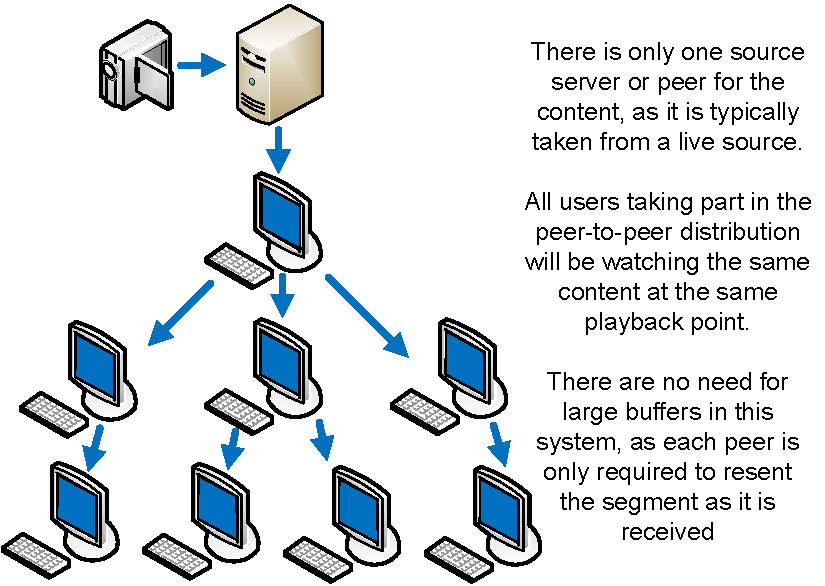
\includegraphics[height=5cm]{./diagrams/P2P-tree}
    }
    \subfloat[][Mesh P2P Network] {
        \label{fig:p2p-mesh}
        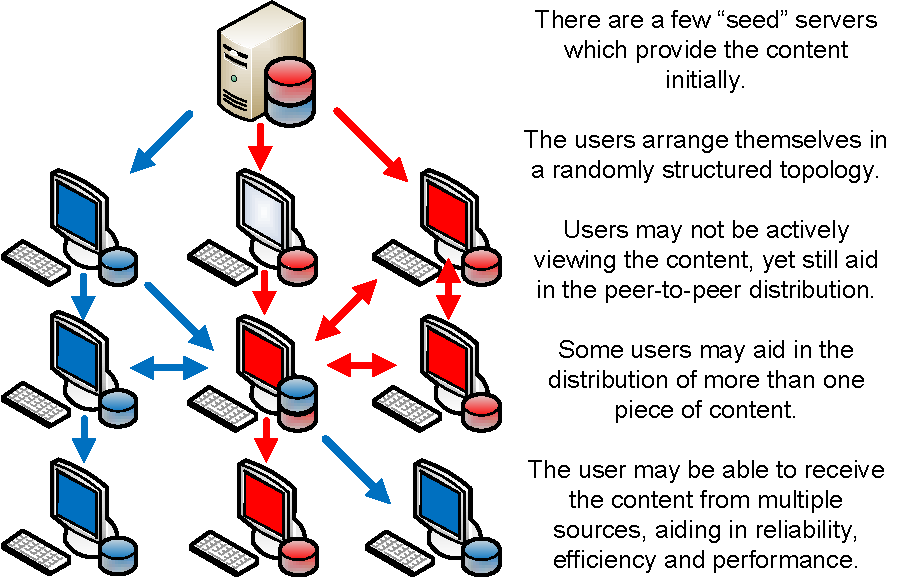
\includegraphics[height=5cm]{./diagrams/P2P-mesh}
    }

    \caption
        [Distribution of media in a peer-to-peer network]
        {Distribution of media in a peer-to-peer network. Different coloured arrows and shapes represent the different content.}
    \label{fig:p2p}
\end{figure}

    Other than the previously mentioned commercial online video-on-demand systems, there are numerous peer-to-peer (P2P) technologies that enable efficient streaming of live and stored media~\cite{liu2008spp,li2007ess}. Traditional P2P has been used to distribute full files~\cite{cohen03ibr,emule,gnutella}, including files such as movies, tv shows, music~\cite{napster}, \emph{etc}. As the full file must be downloaded before playback can begin, this can be considered a primitive form of VoD, similar to that offered by the Kontiki based applications (see \autoref{sect:bbciplayer}).

    After the initial surge of P2P file sharing applications, research began on application level multicast (ALM)~\cite{yeo2004sal}, sometimes called end-system multicast~\cite{chu2002ces}.  This is a form of P2P designed to stream content, in a one-to-many fashion, similar to traditional IP multicast. However, streaming is different to video-on-demand, as all the users are typically viewing the same content at the same playback point.  Video-on-demand should allow users to view different content at different playback points simultaneously, which makes it much more problematic.

    Only recently has research began into the areas of peer-to-peer video-on-demand (P2P-VoD). Using P2P offers many advantages over the traditional client-server approach. Firstly, peer-to-peer can greatly reduce the costs to run the service, as a large CDN is not required to deliver the content. Additionally, in the mesh-based P2P, those able to request from multiple sources simultaneously have advantages when it comes to interacting with the media. These protocols are designed to allow arbitrary segments to be downloaded. Thus, seeking and pausing can occur relatively easily.

    Peer-to-peer does have some disadvantages, such as additional overheads and requiring peers to take part in the delivery. These overheads are from the extra control traffic needed to arrange peers into a structure suitable for media delivery. As peers are the main source of content, they can be less reliable and have less resources than tradition servers. This may result in unpredictable or unreasonable service. Additionally, unless a content protection scheme is used, peers may maliciously alter the content when relaying to other users~\cite{dhungel2007pap}. Also, not all peers have sufficient capacity or want to take part in the network.

    When describing P2P, there are a few different ways the networks may be arranged and how the data is transmitted.
\begin{description}
  \item[Tree] In tree distribution, the peers arrange themselves in a tree, rooted at the source of the content (as depicted in \autoref{fig:p2p-tree}). This is best used for streaming, as there is typically only one source for this kind of content. The content can then be streamed down the tree, and eventually reach every peer. There are many protocols which efficiently arrange peers in this manner~\cite{mathy01otb,banerjee2002sal,tran2003zae}. However, it was noted~\cite{castro2003shb}, if nodes are arranged in a tree, the leaf nodes (those at the bottom) do not distribute to others. This is an obvious waste of resources, as $f^h$ peers within the network do not help distribute the content, where $f$ is the node's out-degree and $h$ is the height of the tree. To better utilise the resource, multi-source trees were developed~\cite{begen2003mps,castro2003shb}. These multi-source trees also make the distribution more robust to failures, such as, a node parent failing~\cite{do2004ppf}. One problem for all trees, is that they may become very deep, causing a high latency (or lag) for the peers near the bottom.

  \item[Mesh] To improve the efficiency of tree based schemes, mesh networks create a seemingly randomly connected graph from the peers~\cite{kostic2003bhb,liao2006app,magharei2007ppp,hei2008iop}, as seen in \autoref{fig:p2p-mesh}. Content may then flow in any direction through this graph, allowing each peer to have many sources, as well as many nodes to share with. This technique is typically used to provide video-on-demand~\cite{annapureddy2006pvd} or file distribution~\cite{cohen03ibr}, as it offers greater reliability and performance, at the cost of additional overheads and less guarantees of the ordering of received data. Unfortunately, peers within a mesh network will experience a higher rate of churn (peers joining and leaving), as each peer is potentially connected to tens of others.
\end{description}

Typically the content is always divided into segments, of fixed (or sometimes variable) size. This allows peers to request individual chunks of the media, as well as to more efficiently inform others which segments they has. The segments are normally either pushed or pulled by the peers though the peer-to-peer network.

\begin{description}
  \item[Push] Push distribution is typically used for live streaming in combination with tree based distribution. In live streaming each peer will require the segments by a similar deadline, and each peer typically only has one parent, the segments can be pushed to the peer, without request. This greatly reduces the overheads of knowing which peer needs which segment, \emph{etc}. Push can also be used in multi-source situations by clever partition tricks, for example, in a two-source situation, a peer can receive odd segments from one peer, and even from the other. However, this gets increasingly complex when there are multiple source peers or the network is in a constant state of churn (as is common in mesh networks).

  \item[Pull] If it is not obvious which peer needs which segment, then pull distribution is better. Each segment must be explicitly requested by the peer before it is sent. This adds additional overheads, but allows the receiving peer to make decisions on where to receive from. Pull is popular in mesh networks, as it simplifies the distribution of content. To allow pull to work, each peer must occasionally share a list of currently buffered segments with their neighbours. This list is typically shared in the form of a bit-map, assigning a one or zero to each segment, indicating whether it is buffered or not.

\end{description}

    This rest of this section discusses the main peer-to-peer systems in both the streaming, and VoD domains.

\subsubsection{Streaming}

    Streaming, is typically used for live events, or broadcasting of traditional style television channels. As such all the users will be viewing the content at the same playback point, as opposed to video-on-demand, which allows users to view different playback points simultaneously.

    There are many commercial peer-to-peer streaming products available, mostly from Chinese companies. These include PPLive~\cite{pplive}, CoolStreaming~\cite{zhang2005cdd}, Zattoo~\cite{zattoo}, TVAnts~\cite{tvants}, PPStream~\cite{ppstream} and SOPCast~\cite{sopcast}. This software has been very popular in China~\cite{fowler2005nef}, and is starting to become more popular in the US/UK.

    CoolStreaming (or more formally known as DONet) was one of the most popular services, when it was in operation. Information about how the system works was made publicly available, and a couple of papers were published on the topic~\cite{zhang2005cdd,xie2007cdt}. However, in 2005 the service stopped broadcasting, less than a year after it first began, due to copyright issues.
% TODO I need a reference for the copyright issue, but I couldn't find one :(

    The CoolStreaming technology is based on a pull mesh-based streaming technique. When joining the system, a newly connecting peer would obtain a list of existing peers from a central repository.  This list would be used to bootstrap the newly connecting peer into the network. Afterwards, a gossip protocol is used to find additional peers. Segments of the media are there pulled from neighbouring peers, who frequently advertise their segment lists.

%   The stream is divided into equally sized segments.  Each peer maintains a local buffer of segments. A list of the peer's segments is occasionally shared in the form of a bit-map, with directly connected peers. Sharing the list allows other peers to know which segments of the stream the peer has. Then, in a pull fashion, a peer can request segments required for its own playback.

    One of the novel features of CoolStreaming is the scheduling algorithm which decides which peer is used for a segment when there are multiple peers to chose from. The problem of deciding the most efficient way for each peer to allocate it's resources is an NP-hard problem, akin to parallel machine scheduling~\cite{cormen2001ita}. Therefore, CoolStreaming uses a simple heuristic to decide the allocation of resources. The algorithm uses a combination of how rare the segment is, how much free bandwidth the remote peer has, and how urgently the segment is needed.

    PPLive~\cite{pplive} is more popular than CoolStreaming, as it has a total of 2.2 million users and 500 different streams~\cite{huang2008cda}. A keynote presentation by Huang, a PPLive Software Architect, demonstrated how scalable P2P streaming can be. In the second quarter of 2007, PPLive supported 1,480,000 simultaneous users viewing the same live sporting event, being served by just one 10Mbit/s server~\cite{huang2007ewp}.

    Even though PPLive is a closed-system it has been a hot-topic for researchers to study~\cite{huang2008cda,silverston2007mpi,vu2007mls,krieger2008aaq,chen2008msc}. Silverston and Fourmaux captured traces from PPLive, and determined it uses a mesh-based pull approach, similar to CoolStreaming~\cite{silverston2007mpi}. Vu~\emph{et~al.} noted that PPLive tries to keep its neighbour peer list around 30 to 45, independent of the number of peers currently taking part in the stream. By keeping the neighbour list around a constant size, this allows the system to scale far more efficiently~\cite{vu2007mls}.

    Vu~\emph{et~al.} also calculated the \emph{clustering coefficient}~\cite{watts1998cds} of this network. This is a measure of how randomly the peers are connected to each other. They found streams with few peers ($<500$ peers) had a high degree of randomness, however, as the stream size increased, many clusters of peers began to form. They did not speculated as to whether the clusters were based on some metric of ``closeness'', \emph{i.e.} network or geographical locality.

    The remaining studies which look at PPLive have looked at simple metrics such as packet size~\cite{krieger2008aaq}, signal overhead~\cite{silverston2007mpi}, stream popularity, and chunk availability~\cite{huang2008cda}. These do not give much insight into how PPLive operates. However, one thing is clear, PPLive is a large peer-to-peer application which has tremendous scaling abilities. This is only let down by the fact that it is a pure streaming application, and does not offer interactivity features beyond pause and resume. Nevertheless, PPLive will encourage development of future projects which take advantage of this form of streaming peer-to-peer, hopefully with addition VoD features.

%Nic has read to here

    % [2] �PPLive�, http://www.pplive.com/.
    % PPLive ( Challenges, Design and Analysis of a Large-scale P2P-VoD System )
    % As of late November 2007, a total of 2.2 million independent users had tried the system. A total of 3900 movies were published in November and December of 2007, with around 500 movies on-line simultaneously. In late January 2008, the number of simultaneous users reached over 150K and was still growing

\subsubsection{Video-on-demand}

    Peer-to-peer video-on-demand (P2P-VoD) typically uses a combinations of P2P file sharing and streaming techniques. Users will contribute local disk space, as well as bandwidth, to allow other users to stream directly from them. Typically the local disks will store multiple videos which have been previously watched, and perhaps a few which have not if the network deemed their replication necessary. Many of the pure streaming techniques can be applied, or slightly altered, to work for video-on-demand. However, this is easiest with the pull based systems, which can easily cope with peers being at different playback points.

    There are a number of commercial systems, such as, Vuze~\cite{vuze}, Joost~\cite{joost} and many others~\cite{gridcast,pfsvod,ppstream,uusee}. Again, all of these systems use proprietary techniques, and as such the only information about them is inferred, or discovered through measurements.

    Vuze, for example, offers a catalogue of thousands of videos, mostly uploaded by users, but some from professional studios. To download the videos Vuze uses a sliding window BitTorrent~\cite{cohen03ibr} technique~\cite{vlavianos2006beb,shah2007ppm}. To begin viewing a video, Vuze must connect to a tracker. The tracker is a centralised server or possibly decentralised in some modern BitTorrent implementation~\cite{roozenburg2006sds}. The tracker maintains a list of all peers who are in the process of downloading, or have finished and now just sharing. The Vuze client uses this list to form a single P2P network for each video.

    Normally, BitTorrent connects to as many peers in the P2P network as possible and begins downloading. Multiple downloads occur in parallel, each requesting a different random segment of the full file\footnote{BitTorrent does not always download segments in a random order, as there are multiple improvements to increase the efficiency of the ordering~\cite{massoulie2005crs}}. The random order helps ensure that the file is spread as quickly as possible throughout the network~\cite{bharambe2005aai}. So that Vuze can display the video to the user as it downloads, it opts to download the segments of the file in a semi-sequential order. A sliding window is created ahead of the playback point, and only segments within this window are downloaded. As playback continues, the window moves along.

    In theory, Vuze could support many interactive controls, however, it only supports pause and resume. Pause is a simple operation as playback from the buffer can stop while not affecting the normal download. Seeking is not possible as time offsets cannot be easily mapped to file segments.  This feature could be added if metadata provided a map of keyframe times to an offset within the file. Then on a seek request the sliding window can be moved to the new seek location, and download/playback resume.

    There are numerous problems with Vuze, for example, the protocol is a very simple modification to BitTorrent, which is not custom-made for this task. This causes the start-up times to be long, and limits the interactive features. Also, because the peer-to-peer networks are only made up of peers who have previously downloaded, or are downloading, the video, it is possible for the video to not be fully available. A more suitable situation would be to either backup the videos on dedicated content servers, or ensure the videos are replicated on nodes with spare capacity, therefore better utilising the network.

    Joost~\cite{joost}, takes a different approach to Vuze, by designing a new P2P-VoD protocol from the ground up. Joost, was created by Niklas Zennstr\"om and Janus Friis, the two entrepreneurs responsible for Skype~\cite{skype} and Kazaa~\cite{kazaa}. Joost has a large catalogue of content, which is provided exclusively by professional studios. Because of Skype's and Kazaa's fame, Joost has been able to secure deals with many large studios, such as FOX networks, Viacom (which includes MTV and Paramount Pictures), and Warner Music. This has allowed Joost to have high quality content, such as feature films and TV episodes.

    Little is know about Joost, however it is reported that it is a mesh based peer-to-peer network backed by servers deployed in a CDN. From one study, it appears that Joost uses UDP packets, to transmit content in MPEG-4/AVC with error-resilience coding~\cite{krieger2008aaq}. It is speculated that Joost will use peers with spare capacity to help distribute content which is popular. This would help to maximise the delivery efficiency.


\subsection{Summary}

% TODO write about this figure!
%\begin{figure}[t]
%    \centering
%    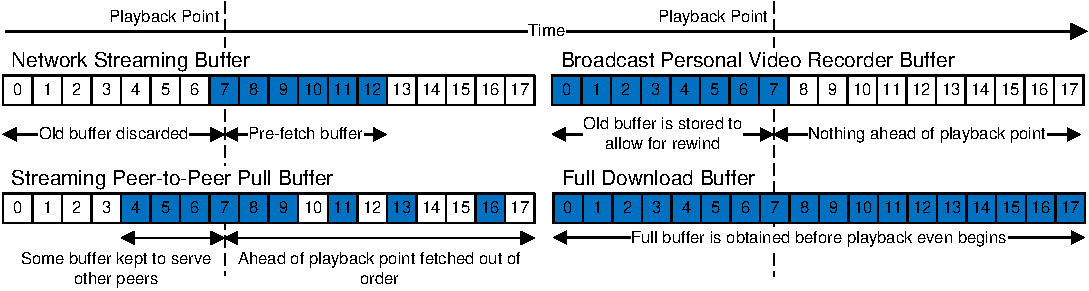
\includegraphics[width=1\columnwidth]{./diagrams/buffers}
%    \caption{Layout of buffers used by various systems}
%    \label{fig:buffers}
%\end{figure}

%\begin{table}[t]
%    \centering
%    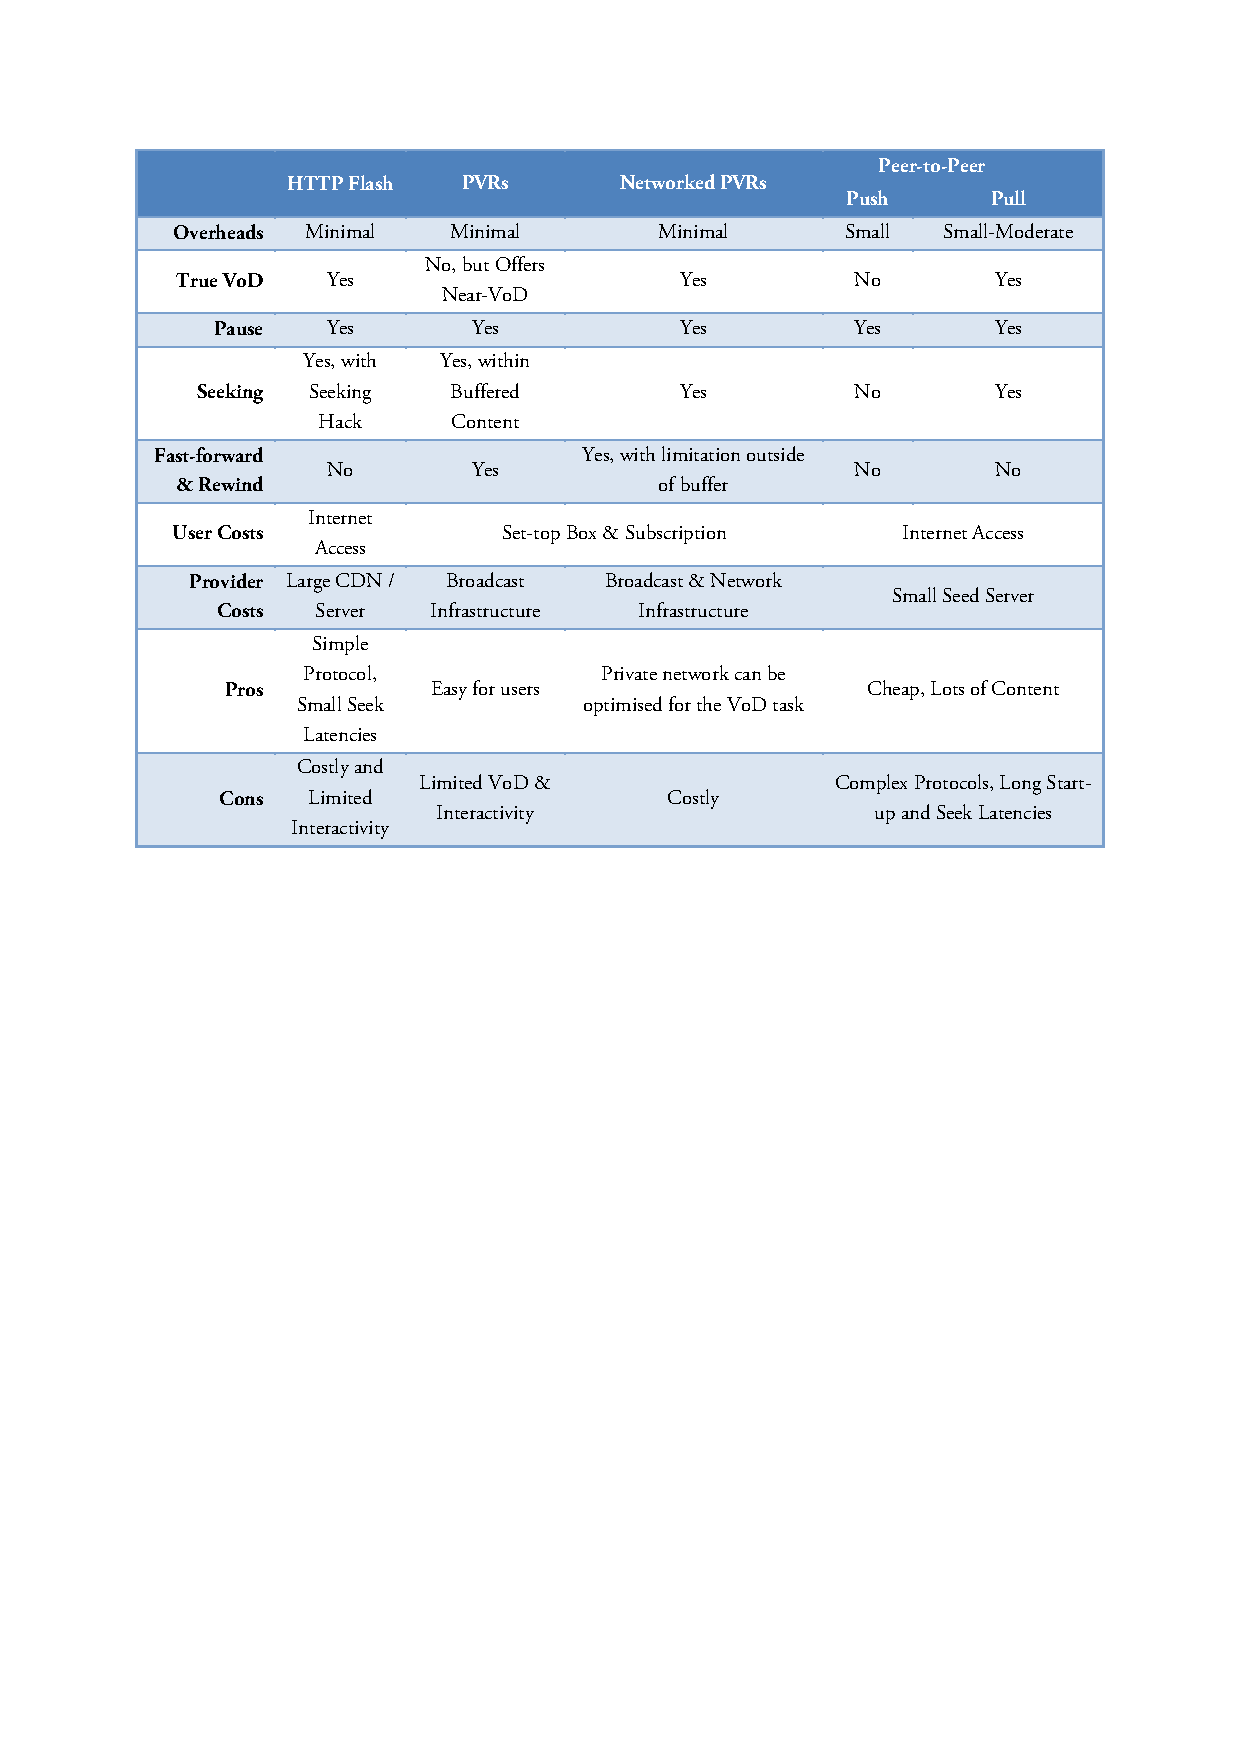
\includegraphics[width=1\columnwidth]{./diagrams/table}
%    \caption{Summary of features available with each video-on-demand system}
%    \label{fig:vod_table}
%\end{table}

\begin{table}[t]
\setlength{\tablecolwidth}{0.14\columnwidth}
\newcolumntype{C}{>{\centering\arraybackslash} m{\tablecolwidth} }
\newcolumntype{R}{>{\raggedleft\bfseries\arraybackslash} m{\tablecolwidth} }
\scriptsize
    \begin{tabular}{|RCCCCC|}
\hline
\setrowcolor{TableRowHead}
                    &  &  & & \cellendbxy{2}{1}{Peer-to-Peer} \\
\setrowcolor{TableRowHead}
                           & \cellbxy{1}{-2}{HTTP Flash} & \cellbxy{1}{-2}{PVR} & \cellbxy{1}{-2}{Networked PVR} & \textbf{Push}   &\textbf{Pull} \\
\hline
\setrowcolor{TableRowA}
    Overheads              & Minimal & Minimal & Minimal &  Small  & Small-Moderate\\
\setrowcolor{TableRowB}
    True VoD               & Yes & No, but offers Near-VoD & Yes & No & Yes\\
\setrowcolor{TableRowA}
    Pause                  & Yes & Yes & Yes & Yes & Yes \\
\setrowcolor{TableRowB}
    Seeking                & Yes, with Seeking Hack & Yes, within Buffered Content & Yes & No & Yes\\
\setrowcolor{TableRowA}
    Fast-forward \& Rewind & No & Yes & Yes, with limitation outside of buffer & No & No \\
\setrowcolor{TableRowB}
    User Costs            & Internet Access & \cellxy{2}{1}{Set-top Box \& Subscription} & \cellendxy{2}{1}{Internet Access} \\
\setrowcolor{TableRowA}
    Provider Costs         & Large CDN / Server & Broadcast Infrastructure & Broadcast \& Network Infrastructure &  \cellendxy{2}{1}{Small Seed Server} \\
\setrowcolor{TableRowB}
    Quality                & Low--Medium & High & High & Medium & Medium \\
\setrowcolor{TableRowA}
    Pros                   & Simple Protocol, Small Seek Latencies & Easy for users & Private network can be optimised for the VoD task  & \cellendxy{2}{1}{Cheap, Lots of Content} \\
\setrowcolor{TableRowB}
    Cons                   & Costly and Limited Interactivity  & Limited VoD \& Interactivity & Costly & \cellendxy{2}{1}{Complex Protocols, Long Start-up and Seek Latencies} \\
\hline
    \end{tabular}
    \caption{Summary of features available with each video-on-demand system}
    \label{fig:vod_table}
\end{table}

%    \todo{Summarise this whole section}
%    \todo{Outline the pros and cons for each concept}
%    \todo{Where do innovation need to come?}

%\begin{itemize}
%  \item Content Distribution
%      \begin{itemize}
%        \item high cost
%        \item low overhead, potentially best service for users
%        \item Can offer interactivity, but extra load on servers
%        \item Simple
%      \end{itemize}
%
%  \item PVRs / Network PVRs
%      \begin{itemize}
%        \item Most integrated, simple for users
%        \item Most be deployed, at cost to the users
%        \item No interactivity unless networked
%        \item Networked has similar problems to CDNs
%      \end{itemize}
%
%  \item Peer-to-Peer
%      \begin{itemize}
%        \item low cost
%        \item high overhead
%        \item Push has lower overheads than pull, but makes it harder to do VoD.
%        \item Users don't want to pay for a server, and upload
%        \item Additional problems, ie stop tampering, seeding own content.
%        \item The pull mechanisms do aid in interactive features
%      \end{itemize}
%\end{itemize}


    The previous sections have outlined popular video-on-demand systems which are currently deployed and in use. Their features have been explained, as well as the pros and cons of using them. Here, we will summarise the previous sections, and aim to discuss the systems compared to each other. To recap, \autoref{fig:vod_table} lists the main categories of systems, and which features they support.

    The HTTP Flash-based systems are typically backed by a content distribution network (CDN), but can in small cases be simple client-server systems. By using a simple \emph{pseudo-streaming} technique, the flash-based web-site is able to provide videos on-demand to a vast audience of users via the internet with minimal overheads and costs to the user. However, the back-end system, will no doubt involve terabytes of replicated data, spread across hundreds if not thousands of servers, typically deployed throughout the world. The cost of running such an infrastructure is not cheap, for example, in 2006 it was estimated that YouTube pays \$1~million a month just for bandwidth costs~\cite{frommer2006ytw}. As such, only the well funded content providers can afford to provide this service.

    Content distribution networks used by Flash-based systems can provide many of the modern interactivity features requested by users, albeit with additional overheads and complications for the servers. The one downside when interacting with these systems is the seek-delay. This is normally quite small (less than 2~seconds), and no longer than a couple of round trip delays, and the time it takes to fetch an initial buffer. This can be reduced by making sure the content servers are near to the end users.

    Personal video recorders (PVRs) are perhaps the simplest system for users, as they integrate with users' existing home entertainment systems. If the content provider is already broadcasting the content, then the cost for deploying the PVRs is just the price of the box. However, a simple broadcast-only PVR does not allow for true VoD, only being able to watch pre-recorded content. To add true VoD, dedicated networks are typically used, which greatly increase the cost for the provider. Regardless, PVRs are able to record content at broadcast quality, which is much higher than that typically found on the internet.

    Finally, the peer-to-peer model of distribution offers the cheapest way to deliver content, and if it is not streamed (and instead downloaded) the highest quality of content. This allows independent movie studios, or amateurs to easily release their work in high-def quality formats. Being cheap comes at the cost of requiring users to aid in the distribution, which typically involves high signalling overheads, for example, to coordinate all the peers in a distributed manner. Aiding in distribution is unappealing to many, as they either have to pay for their bandwidth, or are unwilling to share their resources if they are required to pay for the content or service.

    Peer-to-peer also offers numerous other challenges, which can vastly affect the performance of the system. Unlike with CDNs and PVRs, the relative simplicity of the protocols allows them to have a high level of service and reliability. However, in peer-to-peer, your level of service depends on other users, who join and leave the network as they choose. Also, if a user decides to be malicious, they may disrupt the network, inject illegal content, or tamper with the existing content.

    The added complexity of P2P does allow for higher levels of interactivity. For example, in pull based P2P, the content may be fetched out of order.  It is therefore trivial for the protocol to fetch new seek points, or to even pre-fetch ahead to areas of interest. Features like this reduce seek delay, but this improvement may be negated because of the high overheads and unreliable performance of other peers. There is certainly room for much improvement and innovation to solve the numerous challenges found within P2P.

%\todo{Some how get my story across}

%\subsection{Motivation}
%%    \item Discussion on Interactivity and how it breaks streaming
%%    \begin{itemize}
%%        \item Introduction
%%        \item Push/Pull Techniques~\footnote{incorporating Andy's Hybrid work.}\saveFN\andy\
%%        \item Hybrid concepts~\useFN\andy\
%%    \end{itemize}
%
%    "Exploring prefetching to improve the scalability of these protocols for interactive workloads is left for future work."~\cite{costa2004aci}


\section{Characterisations of User Behaviour}
\label{sect:characterisations}

%todo add some diagrams to explain the models

%\todo{Add a interactivity spin, to make it clear we need to understand interactions}

%"can help in designing and evaluating call admission strategies [3], scalable compression techniques [18], and client/server buffer management strategies [4] for CM systems"~\cite{padhye1999cmc}

To design systems that support the delivery of multimedia over the internet, it is crucial to understand how users will interact with the media. These interactions impact multiple functions, such as, admission strategies, buffer management and delivery techniques.

In a content distribution networks (CDNs) context, this could effect how proxy servers operate, and how the location of replicated media, and which delivery mechanisms are used. If, for example, only a small subset of media from a large catalogue is popular then more resources should be dedicated to those popular files. Content could also replicate in advance, if it was possible to anticipate demand. This is all possible by understanding how the content is consumed by the user.

One area which has not been closely examined, is when there are high levels of interaction, such as those when a user wishes to view just the highlights of the content, or is searching for a specific clip. Understanding highly interactive characteristics can aid in the designs of many novel features. This may include the ability to pre-fetch areas of high popularity, or place bookmarks at key points.

The behaviour of users has previously been studied in a few different domains, including static web content, video-on-demand, and live streaming. Each have different properties, causing the observed user behaviour to differ for each domain.

Video-on-demand (VoD) domain consists of applications in which videos from a stored catalogue can be fetched and viewed at the user's discretion. These applications typically allows the user to control the playback of the content, for example, allowing users to pause, fast-forward, or rewind. Live streaming is akin to TV broadcasting; all users viewing a particular stream do so at same playback point, thus limiting their control over playback.

Veloso~\emph{et~al.} describe VoD as \emph{user driven}, meaning that the user decides which media is viewed and when. However, live streaming is \emph{object driven}; the user's access is influenced by show/event time, and the various activities within the live media~\cite{veloso2002hcl}.

%Within this section the behaviours of users will be characterised for the different domains.

%\subsection{Web Content}
%fetch-at-most-once

\subsection{Video-on-Demand}

    The characterisation of Video-on-demand (VoD) is important to this thesis, as the main experiments involved VoD. As such it is important to have a understand of existing VoD characterisations, to contrast with the new results found within this thesis. Additionally VoD has become increasingly popular over the internet, and is thus introducing new challenges which need solving. Already, 11\% of people within the UK supplement or replace their broadcast TV viewing with online video services~\cite{YouGov2008red}.

%    A study conducted on the University of Washington campus found that 85\% of all streaming sessions were for Video-on-Demand content, the remaining 15\% therefore belonging to Live Streaming~\cite{chesire2001maa}.
    In a 2001 study, the streaming habits of users on the University of Washington campus were recorded. It was found that 85\% of all videos viewed were from stored content~\cite{chesire2001maa}. This percentage is thought to have increased as numerous video websites have become very popular, with YouTube~\cite{youtube}, for example, receiving 70 million visitors a month~\cite{saxena2008avs}.

    Multiple studies have suggested that the majority of online VoD content is relatively short~\cite{li2005csm}, with 93\% of content having a duration of less than 10 minutes~\cite{chesire2001maa}, and a median of 3.2-3.9 minutes~\cite{saxena2008avs}. The length of video content is expected to increase as VoD becomes more popular driven by services such as BBC iPlayer~\cite{iplayer} offering TV shows and feature films.

    %This has already started to happen with a 2008 study of the UK's viewing habits indicating that 11\% of people use online services to supplements or replaces broadcast TV viewing~\cite{YouGov2008red}.

\subsubsection{Popularity}

\begin{figure}[t]
    \centering

    \subfloat[][Zipf distribution: The $i$\sth rank occurs $1/i^\alpha$ of the time. This gives the appearance of a straight line on a log-log plot]{
        \label{fig:dist_zipf}
        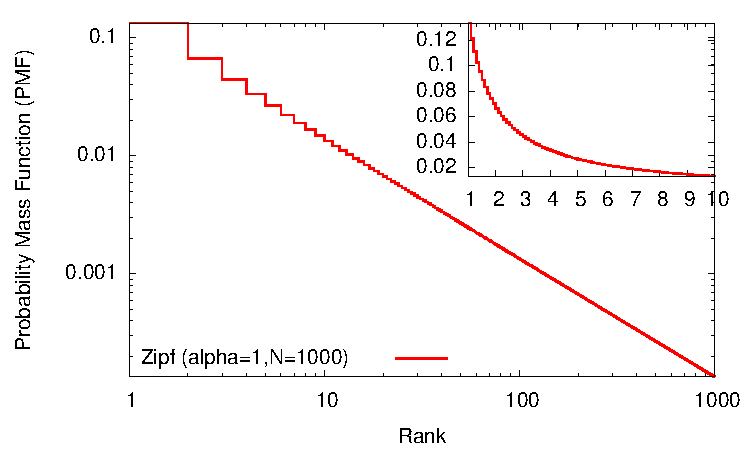
\includegraphics[width=0.45\columnwidth]{./diagrams/powerlaw-zipf}
    }\qquad
    \subfloat[][Pareto distribution: This follows the 80-20 rule, where 80\% of the function's weight is within the top 20\%] {
        \label{fig:dist_pareto}
        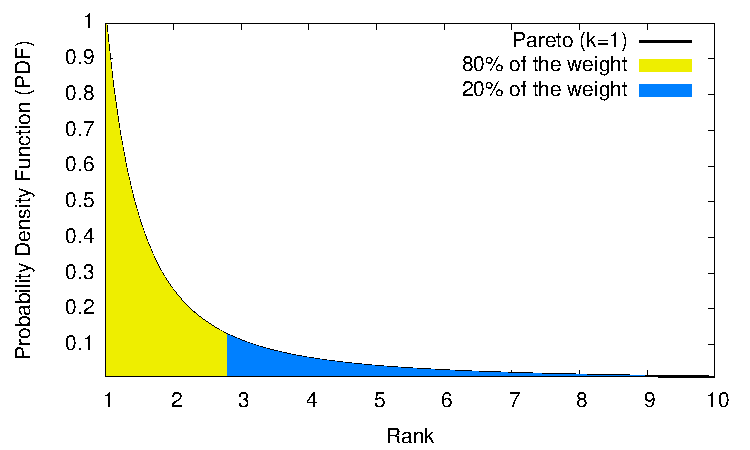
\includegraphics[width=0.45\columnwidth]{./diagrams/powerlaw-pareto}
    }

    \caption
        {Probability density functions for Zipf and Pareto distributions}
    \label{fig:dist}
\end{figure}

%   "Temporal Locality: accesses to videos also exhibit strong temporal locality. If a video has been accessed recently, chances are that it will be accessed again soon."~\cite{acharya2000cua}

%   "Our analysis found that of the 23,738 media objects referenced, 78\% were accessed only once. Only 1\% of the objects were accessed by ten or more sessions, and the 12 most popular objects were accessed more than 100 times each."~\cite{chesire2001maa}.

    The popularity of content within a VoD system play an important role in deciding how it is cached and replicated. Popularity of web objects typically follow a Zipf-like distribution. Within Zipf distributions~\cite{zipf1949hbp}, the popularity of a object is proportional to its rank, \emph{i.e.} the $i$\sth most popular object receives $1/i^\alpha$ of requests, as seen in \autoref{fig:dist_zipf}. This implies the majority of content is unpopular, and a few items are extremely popular, making up the weight of the distribution. This is be illustrated by observations made by Chesire~\emph{et~al}. Out of 23,738 video objects, 78\% of which were only accessed once, 21\% accessed two to nine times, and the remaining 1\% accessed ten or more times, with the 12 most popular objects being accessed more than 100 times each~\cite{chesire2001maa}.

    Video-on-demand popularity was first suggested to follow a Zipf distribution by Dan~\emph{et~al.} in 1994~\cite{dan1994spf}. This was again observed by Wolf~\emph{et~al.} in 1997, however with varying degrees of skew each week~\cite{griwodz1997ltm}. In early 2000, Acharya~\emph{et~al.} could not fit the popularity of their education videos to a Zipfian distribution~\cite{acharya2000cua}. Instead they noticed requests to their objects were more biased towards the popular titles than expected within a Zipf distribution. This bias can be explained by Cherkasova and Gupta's analysis of an enterprise media workload~\cite{cherkasova2002cle}. They observed that over long timescales the bias towards the most popular items increased. For example, object popularity fitted a Zipf distribution with $1.3 \leq \alpha \leq 1.6$ over 1-month periods, over a 6-month period with $\alpha=1.6$, and eventually Zipf did not fit well over a year.

    The fact that Zipf did not fit well over a year time scale is often overlooked and the reasons for this are typically misunderstood. Zipfian models are useful for static distribution, those which do not have a temporal component. For example, Zipf was first developed by George Kingsley Zipf when studying the frequency of words appearing in a corpus of natural language. The corpus would not change over time, \emph{i.e.} words would not be added or removed. This differs from popularity of videos over a timescale as it is common for new videos to be added and removed over time, and for the popularity of the videos to change over time. Instead the Zipf models should be used to model the popularity over shorter periods, such as daily or weekly, or be used to blindly model the rank of objects on daily bases. For example, objects on a daily bases may follow a Zipf distribution, but instead of noting the popularity of each object, note the popularity of each rank. This will then more accurately model the expected popularity on any given day, and is more useful for the design of caching systems.

    % Maybe mention why web objects are requested multiple times (ie they change)

    Whilst analysing Kazaa's~\cite{kazaa} peer-to-peer traffic, Gummadi~\emph{et~al.} proposed a new distribution that fitted the popularity of objects better than Zipf~\cite{gummadi2003mma}. Individual Kazaa users rarely requested the same object twice, unlike in web traffic where the same object may be requested multiple times by an individual. This lead to the ``fetch-at-most-once'' model, which fitted better to the workloads discussed by Cherkasova and Gupta~\cite{cherkasova2002cle}, as well as ranking data collected from video store rentals~\cite{vsm}, and box office sales~\cite{imdb}. This model says that users fetch objects following a Zipf distribution, but must not request the same object twice. If the user chooses a previously fetched object, then a new object is picked again from the Zipf distribution.

%\todo{Find who compared fetch-at-most-once to video rentals}

    Yu~\emph{et~al.} contradicted the fetch-at-most-once model when analysing a 219 day trace collected from a VoD system deployed by China Telecom used by 150,000 people~\cite{yu2006uub}. Their object popularity fitted best to a Zipf distribution, except for a long heavy tail. They speculate that their results do not fit the fetch-at-most-once model because users were unable to save the viewed media, thus if they wished to watch a video again, they had no choice but to re-fetch it.

    Which model is best seems to depend on how the videos are accessed, what genre of video they are, and other currently unknown factors. However Cha~\emph{et~al.} tried to explain the shape of the distributions through simulation~\cite{cha2007tyt}. A fetch-at-most-once model was simulated with a Zipf distribution of $\alpha=1.0$. Parameters such as the number of users, the number of requests per user, and the number of objects were varied. They found that the effects of fetch-at-most-once are barely noticeable when there are few requests, this intuitively makes sense as there is less chance of selecting the same object twice. The number of users did not seem to impact the shape of the distribution at all. When the number of objects increased, the effects of fetch-at-most-once were also reduced, again, because the chance of selecting the same object is decreased.

    Both Zipf and fetch-at-most-once are categorised as power-law distributions. However there are other factors which govern the power-law nature of these distributions. In most of the analysed models, the two ends of the distributions have been truncated or extended. It is suggested by Chris Anderson that ``Latent demand for products ... is suppressed by bottlenecks in the system''~\cite{anderson2006tlt}. Take, for example, the popularity of movies in cinemas. Most cinemas show the most popular movies, however there are few cinemas screening niche content. This causes the popularity distributions of the movies to have a truncated tail. This is refereed to as a ``distribution bottleneck'', where due to lack of distribution, the tail is truncated. The opposite can be true, where, for example, there is ample supply of niche content, but it is hard to find this niche content, thus a ``information bottleneck'' exists~\cite{cha2007tyt}.

    %TODO Perhaps a last paragraph to summarise?

\subsubsection{Popularity Over Time}
\label{sect:pop_over_time}
%    Popularity is greatly changed by top-ten lists~\cite{yu2006uub}
%    Popularity changes each day as new content is added~\cite{paneda2006pav}
%    The content is divided into many groups: "Short life", "Long life", "Up and down", "Seasonal"~\cite{paneda2006pav}
    Over time the popularity of videos will change, greatly impacting the decision on what to cache or replicate. It is essential to consider how frequently replication updates are carried out. Too often and video may needlessly be moved, but too infrequent and the servers may not be prepared for demand of a newly popular video. As such the rate of change in user interest can aid in the design of a VoD system.

    Paneda~\emph{et~al.} noted the popularity of videos on a popular Spanish news website would change daily as new content was added. Typically the most popular items for each day were added to the site on that day. However after the first day the content could be grouped into four categories; \emph{short life}, \emph{long life}, \emph{up and down} and \emph{seasonal}. Short life content would reach its peak popularity on the first day, and after the first day the number of accesses would decrease suddenly. Long life content also peaks on the first day, however its popularity decreases slowly over the the following days/weeks. Up and down content, will build up popularity for a few days, and then decrease in a similar way to long life. Finally, seasonal content would have peaks in popularity every few weeks or months~\cite{paneda2006pav}.

    In a study of a enterprise media server, Cherkasova and Gupta observed that on any given month most of the bytes transferred were for new content. They found that \verb+~+50\% of requests to content were made in the their first week, with and addition 20\% to 30\% being made in the following four weeks~\cite{cherkasova2004aoe}. They did not discuss if they found seasonal or \emph{up and down} style content. However these patterns may be directly related to the genre or appeal of the content.

    Yu~\emph{et~al.} took a different approach to monitoring popularity over time in their large scale VoD system~\cite{yu2006uub}. They looked at the rate of churn in the top-10, top-100, and top-200 most popularity movie charts over different time scale. They began by looking how newly inserted content affected these top charts on a hourly timescale. The time content was added to the system, correlated with a high change in user interest. This encourages that newly added content be replicated early to avoid insufficient availability.

    It was also noted, that over a small time scale, \emph{i.e} hours, the top-10 list had a small amount of churn averaging around 25\% change per hour, whereas the top-100 and top-200 experienced 45\% change per hour. Over longer timescales such as days and week, it was found that the top-10 list rarely remained stable, whereas the top-100 changed only 15\% each day.

    The main observations from Yu~\emph{et~al.} suggest that popularity changes on different timescales, with the top-10 being stable for a day, and the top-100 being stable over longer periods. It is suggested that a two level caching model be used, with a small adaptive cache for the top-10, and larger more constant cache for the top-100~\cite{paneda2006pav}.

    Although popularity of objects change over time, it appears these changes are very specific to the viewing population and genres of the objects. In the current research no single model has been found which accurately explain the observed behaviours, however, it is clear that this is an important metric for cache design.

\subsubsection{Recommendations}

% TODO Fix the below paragraph
    Some systems display a top-10 list of the most popular videos that month, or a list of recommendations, such as new releases, or videos a user may find of interest. All of these lists can greatly influence what a user views. However, the importance of recommendations has not been studied, much, it has been highlighted as a great source of revenue for companies such as Amazon~\cite{anderson2006tlt}.

    Yu~\emph{et~al.} have studied this phenomenon more analytically when they observed it in their VoD system. They found one video stayed in the top-15 most popular film list for a significant amount of time, but once a administrator manually removed the film from the list, its popularity quickly declined~\cite{yu2006uub}, and never recovered.

    The fact that users appear influenced by these lists, can play in the favour of a video-on-demand system. For example, if it is know ahead of time that a film will appear in the list, the system can take necessary steps to ensure the content is well replicated, in advance of the demand.

%This factor can also impact the results later shown in this thesis. We displayed a list of bookmarks to the user, and found them to be very popular.

\subsubsection{Session duration}

    The session duration can be defined in two ways; firstly the duration a user spends using a Video-on-Demand application, and secondly the duration the user spends watching a particular video. Each definition is applicable in different contexts. For example, knowing how long a user views a single video can aid in caching decisions, whereas knowing how long a user uses an application can aid in the design of the application. This section is only interested in how long a user views a particular video for.

    From early studies on VoD it has been observed that session duration is quite short. For example, in 2001, whilst studying streaming traffic on a large university campus, Chesire~\emph{et~al.} showed that 85\% of all sessions lasted less than 5 minutes with a median session duration of 2.2 minutes. This is compared to a mean advertised media length of between 2.5 and 4.5 minutes. Long lived sessions (those longer than one hour) accounted for only 3\% of all client sessions~\cite{chesire2001maa}.

    Almeida~\emph{et~al.} found similar results when analysing logs from an educational media server. A significant proportion of requests were less than 3 minutes in duration. These sessions were very short when compared to the length of the media, which had a median length of 60 minutes~\cite{almeida2001aem}.

    %Padhye and Kurose also looked at an educational media service, which provided HTML lecture slides, accumplied with audio narration. The session direction of

    It was suggested by Guo~\emph{et~al.} that the short duration was due to the long wait times, and low patience of users~\cite{guo2005amw}. Yu~\emph{et~al.} found that short durations within their traces were due to users sampling the media by ``scanning'' through them. An inverse correlation was also found between the session lengths and the popularity of the media. Less popular videos actually had longer session times~\cite{yu2006uub}.

    As noted by Guo~\emph{et~al.}, 20\% of network bandwidth was wasted buffering video which was never watched due to the user aborting the stream~\cite{guo2005amw}. These short session durations encourage the design of agile systems which can quickly display the media before the user becomes impatient, as well as techniques such as prefix caching~\cite{sen99ppc}, which prioritise caching of the first frames of the media for quick delivery.

\subsubsection{Interactivity}

    % Describe what interactivity is, and why its important
    % Few people interact
    % longer files have more interactivity, also with longer files more forwards are noticed, and less pauses

    % Pause is the most common
    % Jump forward and back are equally popular

    % TODO Find that paper with short/medium/high interactivity levels

    The playback of media is not always passive; certain systems allow for interactive control over the playback. For example, the user may be able to pause, fast-forward or rewind, as well as seek to arbitrary points within the content. Offering interactive features can be challenging. For example, most multicast delivery techniques require all clients to be at a similar playback point within the stream. However, if a client seeks arbitrarily, they are no longer at the same playback point, and thus must join another multicast group, or start to receive the content via a different delivery method. As such, an understanding of how users interact with the content can be invaluable for good delivery.

    There have been few studies on how users interact with media. This may be due to the relatively few systems which have interactive features. However, Huang~\emph{et~al.} found then when interactive controls were available, for videos clips shorter than 30~minutes, only 20\% of all sessions showed interaction from users~\cite{huang2007civ}. Unsurprisingly, the longer the video, the more interactivity is observed. For example, with videos less than a hour in length 40\% of session exhibited interactivity. This trend is consistent with the results within this thesis, and other research~\cite{costa2004aci}. However, this thesis presents results with far higher percentage of sessions with interactivity. This may be due, in part, to the novel interface presented to the users which encouraged interactivity.

    Costa~\emph{et~al.} found that when users do interact, that in both education and entertainment the most common action is pause~\cite{costa2004aci}. This was confirmed by Vilas~\emph{et~al.} who noted that 7\% of session for short videos (those less than 5 minutes in length) and 10\% of longer videos session had at least one pause. It was also shown that the pause duration could be modelled with a Weibull distribution, with means of 55 seconds and 95 seconds, for short and long videos respectively~\cite{vilas2005uba}.

    Another common action is seeking forwards or backwards. For short videos, the percentage of forward and backwards seeks appeared to be roughly the same. However as video length increases, there are more forward seeks, indicating users wished to skip ahead~\cite{almeida2001aem}. Seeking forward also surprised Padhye and Kurose when studying an education server which provided lectures. They assumed students would regularly seek backwards to go over a section again, but found that seeking forward was seven times more popular than seeking backwards~\cite{padhye1998esc}.

    Vilas~\emph{et~al.} modelled the number of seeks per session, and follow it matched a Zipf distribution, with $\alpha$ values between $3.73$ and $5.8$~\cite{vilas2005uba}. This implies that most users never sought backwards or forwards, however when users did, they did so numerous times.

    %\todo{A paper somewhere talks about bursts of seeks, and then long playbacks, and then a burst again}

    The distance sought was also studied by Padhye and Kurose, who observed on their education server a very large average distance. For forward seeks this was approximately 35 minutes, and backward was 34 minutes, for media around 70 minutes in length. However, one third of these seeks were for less than 3 minutes~\cite{padhye1999cmc}.

%\todo{Talk about ON/OFF time analysis}

%    7\% of short video sessions had 1 or more paues, and 10\% of long videos had 1 or more.~\cite{vilas2005uba}
%    Pause length 55.7s and 95s for short and long respectivitly
%    Shows slightly more forward than back jumps

%    short videos (0-5 min)
%    long videos (5-50 min).
%
%    Forward (short videos) Zipf ? = 5.8 = mean 1.0226
%    Forward (long videos) Zipf ? = 4.32 mean 1.0808
%    Backward (short videos) Zipf ? = 4.32 mean 1.0808
%    Backward (long videos) Zipf ? = 3.73 mean 1.1469
%
%Forward (short videos) Weibull alpha =0.16827 beta =0.45321 mean 124.4929s
%Forward (long videos) Weibull alpha =0.10916 beta =0.54129 mean 104.4828
%Backward (short videos) Weibull alpha =0.09058 beta =0.47459 mean 348.7646
%Backward (long videos) Weibull alpha =0.059598 beta =0.59236 mean 178.7992
%
%    During periods of approximately stationary request arrival rate, the BIBS client session arrival process is approximately Poisson, whereas the time between interactive requests within eTeach sessions is more accurately modeled by the heavy-tailed Pareto distribution, as has been found in more traditional Web server workloads [3,16, 19].~\cite{almeida2001aem}
%
%    Fast forward and rewind operations are extremely rare in eTeach (i.e., less than 0.5\% of all requests in the logs)~\cite{almeida2001aem}
%
%    "For short files, jump backwards is the most common client interaction. For larger file sizes, pauses become more frequent"~\cite{almeida2001aem}
%
%    "Pause is, by far, the most common client interaction in the video workloads. Jump backwards and jump forwards are roughly equally frequent for longer videos."~\cite{costa2004aci}
%
%    Unsurprisingly longer files have more interactive requests~\cite{costa2004aci}
%
%    "As file size increases, the percentage of pauses decreases, and the percentage of jump forwards increases. In other words, clients tend to skip more uninteresting file segments as they watch longer videos. The frequency of jump backwards remains roughly stable across all file size ranges in both workloads"~\cite{costa2004aci}
%
%    "a client usually interacts with the video in the same way repeatedly"~\cite{costa2004aci}
%
%    "average jump distances in either direction increase with file sizes"~\cite{costa2004aci}

\subsubsection{Segment Popularity}

%    For the most frequently accessed files in eTeach, all ten-second segments of the media are accessed nearly equally often, whereas for less popular files, the access frequency is higher for earlier segments of the media.~\cite{almeida2001aem}

%    "It is roughly uniform for the most popular files (usually lectures above 15 minute long), as shown in Figure 12-a, and skewed towards early segments for less popular files, as in Figure 12-b."~\cite{costa2004aci}

%    "If it is roughly uniform (as in Figure 12-a), a single (file) measure is enough to capture the distribution of segment access frequencies, and full file caching is the best strategy for unicast delivery. In the cases where a skewed distribution was found, the curve is usually well behaved (as shown in Figure 12-b) and can be roughly approximated using only two or three measures."~\cite{costa2004aci}

    When users seek, not all segments of the video may be viewed equally. This could lead to some segments being very popular, whereas others unpopular. This situation can also be caused if users do not watch for the full duration of the video. This all has implications on how media, or segments of the media should be cached.

    Almeida~\emph{et~al.} divided education media into ten-second segments. For the most popular video, all segments were accessed roughly equally, however for the less popular video, the earlier segments within the media were accessed more~\cite{almeida2001aem}. This indicates only the beginning of the content was viewed. Costa~\emph{et~al.} also observed this result with newer education content, as well as entertainment content~\cite{costa2004aci}.

    When Huang~\emph{et~al.} analysed the traces from a large entertainment Video-on-Demand site, they found users would regularly quit before the end of the video. For short videos, most users watched for the full duration, however as the video length increased users were more likely to stop early. For example, with videos less than 30~minutes in length, only 18\% would watch for the full duration, with 22\% watching for 60\% of the duration~\cite{huang2007civ}.

    % A similar finding was made by Cherkasova and Gupta when they observed

    These later results are consistent with the findings in this thesis, however, we noted areas of high interest dubbed \emph{hotspots}. The previous work found only minor differences in segment popularity, whereas we found segments with orders of magnitude different popularity. This result is speculated to be because of the higher levels of interactivity found within this thesis' traces.

\subsection{Live Streaming}

% vandermerwe2002svt     Streaming video traffic: Characterization and network impact
% veloso2006hcl          A hierarchical characterization of a live streaming media workload
% sripanidkulchai2004als An analysis of live streaming workloads on the internet
% li2005csm              Characteristics of streaming media stored on the Internet
% chesire2001maa         Measurement and analysis of a streaming media workload
% costa2004aci           Analyzing client interactivity in streaming media

%   In such an environment, users are mostly �passive�; they are fairly limited in how they are allowed to interact with objects: they can only join or leave the audience of the live �active� object."~\cite{veloso2002hcl}

    % Nic has read below

    The characterised workloads of live streaming are likely to be different to those of video-on-demand for a couple of reasons. Firstly, users are mostly passive in live streaming, fairly limited by how they can interact with the media. In some cases, pause is available, but seeking is typically not. The only real interaction available is the choice of when to join or leave the stream. Also, as all users are viewing the same content, the force of the crowd may be stronger, for example, all user leaving simultaneously as a live programme ends.

    Secondly, in a 2004 study of a large CDN, it was found that only 7\% of streams were video, accounting for only 1\% of all requests~\cite{sripanidkulchai2004als}. The remaining streams were audio only, for example, radio stations. This section highlights the differences between VoD and live streaming workloads, while explaining any features specific to live streaming.

%\subsubsection{Popularity - Both VoD and Streaming}
%    \todo{start/finish}
%
%        "The distribution of client requests to objects (in both VoD and Streaming) is Zipf-like, with a alpha parameter of 0.47."~\cite{chesire2001maa}.
%
%        "Accesses to pre-recorded, stored media objects are user driven;3 they are directly influenced by user preferences� namely, what to access and when to do so. Accesses to live media are object driven; they are directly influenced by aspects related to the nature of the object�e.g., show/event time, activities captured by various feeds, etc. In such an environment, users are mostly �passive�; they are fairly limited in how they are allowed to interact with objects: they can only join or leave the audience of the live �active� object."~\cite{veloso2002hcl}

%    \subsubsection{Popularity}
%        The popularity distribution is Zipf-like with two distinct modes~\cite{sripanidkulchai2004als}.

\subsubsection{Time-of-day}

    % Non-stop streams had daily periodic access patterns
    % Patterns followed user's timezone
    % Short streams however did not follow any time-of-day access
    % Short streams did however always start with a flash crowd. Indicating object driven requests
    % Almost 50\% of non-stop streams also had flash crowds, on some days.

    Non-stop streams have a diurnal access pattern, peaking at the same time each day. This kind of diurnal access patterns has not be observed with Video-on-Demand. It is speculated by Veloso~\emph{et~al.} that diurnal access patterns are smoothed out because the clients have control over when they access the media and by clients accessing from multiple time zones~\cite{veloso2006hcl}. The non-stop stream is also influence by time zones, but less so, for example, Sripanidkulchai~\emph{et~al.} observed for a single radio station's stream, several similar periodic patterns were present, but shifted by the time zone of the clients~\cite{sripanidkulchai2004als}.

%Nic has read below

    Streams with a short durations did not follow the same daily pattern. However, nearly all short stream began with a \emph{flash crowd}. A flash crowd is a sudden surge of users all wishing the view the same content. This typically overwhelms servers, and results in an accidental denial of service. These types of events are certainly \emph{user driven}, with users specifically joining the stream for an event. Almost 50\% of non-stop streams also exhibited a flash crowd event every few days. This, for example, could be the result of many users joining a radio stream to listen to a popular programme~\cite{sripanidkulchai2004als}. This behaviour is rarely seen in VoD systems, as the requests are \emph{object driven}.

\subsubsection{Session duration}
%Nic has read below

    Session durations for live streaming follow that of video-on-demand. Most sessions are short, with a a few long-lived sessions. Vandermerwe~\emph{et~al.} found the distribution of session duration to be long-tailed, with 69\% of sessions being less than 2~minutes in length, 88\% less than 10~minutes, and the top 8\% being longer than 20~minutes~\cite{vandermerwe2002svt}. These results were similar to Chesire~\emph{et~al.} who found a similar long-tailed distribution with their top 3\% of the population being more than a hour in length. However, these 3\% of long-lived sessions accounted for about half of all bandwidth consumed~\cite{chesire2001maa}. This demonstrates how the distribution is not just long-tailed, but heavy-tailed.

    Sripanidkulchai~\emph{et~al.} compared the session durations of live streaming content, repeating streaming content and video-on-demand content. The repeating streaming content consisted of non-stop streams which broadcasted the same programme over and over, for example, every 30~minutes. The session duration for both repeating streaming content and the VoD content exhibited similar ``truncated'' Pareto distributions. The majority of sessions with this distribution are short, with the few long-lived sessions being no longer than the content's length. However, the session durations for live streaming content, fitted a Pareto distribution with a heavy tail. This extended long tail is caused by the user's actions, rather than being truncated arbitrarily by the content's length~\cite{sripanidkulchai2004als}.

% ~\cite{chesire2001maa}
% Although the long-lived sessions ( > 1 hour) account for only 3\% of all client sessions, these sessions account for about half of the bandwidth consumed by the workload

% ~\cite{vandermerwe2002svt}
% A large proportion of the sessions (69\%) are on for 2 minutes or less. However the distribution exhibits a long tail About 12\% of the sessions are at least 10 minutes long, while 8\% of the sessions are longer than 20 minutes.

% ~\cite{sripanidkulchai2004als}
% Session duration distributions are heavy-tailed. The tails have 3 distinct shapes corresponding to 3 types of streams: nonstop with fresh content, non-stop with cyclic content, and short streams.

\subsubsection{Interactivity}
%Nic has read

    As far as we are aware there have been no studies on the characterisation of interactivity with live streaming. This will of course be due to the lack of interactive controls. For example, it is impossible to seek forward in a live stream, and only possible to seek backwards if the stream has been stored by the server or client.

    The storing of live streams by the client is becoming increasingly popular with the use of \emph{time-shifting} devices such as digital video recorders (DVRs) or personal video recorders (PVRs). These are typically set-top boxes which buffer broadcast TV. The user is then able to pause while the box continues to buffer, or rewind within the buffer. Additionally, the user may fast-forward to catch up with the stream if they have paused or rewound. PVRs are discussed in more detail in \autoref{sect:pvr}.

    As far as this author is aware, there have been no research examining how users interact with PVRs. However, it is commonly reported that these devices are used to fast-forward through advertising when watching recorded programming~\cite{barwise2005ffp}. When users skip adverts, these advertising segments become less popular than the rest. This has implications for how these segments would be cached or replicated.

%    "More than half (57\%) of all UK residents �time-shift� their TV viewing, using on-demand TV services or recording live television for viewing later", "36\% use a PVR"~\cite{YouGov2008red}

\subsection{Implications}

%Nic has read

%    "Such insight is useful for system design, evaluation, planning, and management"~\cite{sripanidkulchai2004als},

%    "Therefore, system caches can maximize their effectiveness by allocating the majority of their capacity to storing beginning segments of movies." ... "Clearly, VOD systems need to exploit time-varying user interest patterns by intelligently partitioning videos into segments and taking their time index in replica and cache management."~\cite{yu2006uub}

    This section has highlighted the main characterisation models for both video-on-demand and live streaming. Understanding how media is consumed has many practical uses, such as designing, evaluating, planning and managing systems. This is especially true when dealing with highly interactivity workloads, as these typically cause excessive load for servers.

    It is clear that starting with a metric as simple as content popularity can greatly aid in replication and caching strategies. As popularity is typically modelled by a power-law distribution, systems will benefit from caching the most popular content. However, as distribution bottlenecks are reduced, and users find it easier to access their niche content, it might be useful to implement multi-level caching hierarchies, which can use different policies based on the the ranking of the content. For example, one caching policy can be used for most popular content, whilst another can be used for the more niche content. As such, the niche caching policy may only store the content in local caches for a short, whereas the very popular content is kept available for a longer period of time, on a more global scale.

    Knowing what is popular, and caching it, is a reactive method, however, it is sometimes useful to be proactive. This may be possible if the content is listed in top-x charts, such as the top-10 voted movies. The popularity of an object ranked 10\sth, is far higher than that at position 11, when only the top-10 chart is available to the user. The effect these charts have on the user's viewing habits can easily be exploited by the video-on-demand system. As soon as the chart is available, the system can begin pro-actively replicating the content, perhaps near to the target demographic.

    It is also clear that certain content has a seasonal or recurring monthly appeal, such as Christmas-themed videos. Again, these can be pro-actively replicated ahead of demand, at the cost of potentially wasting resources. Other content is perhaps only popular for a very short time, such as daily news reports. Understanding the appeal of the media can greatly help choose on the appropriate content management techniques.

    Where interactivity is concerned, it is already clear that users can be impatient and either scan through the content, or prematurely stop playback. Therefore, to maximise caching efficiently, the first segments of media can be stored in preference to the later segments. Techniques such as prefix caching~\cite{sen99ppc,hofmann1999cts} can also aid in deciding which segments are the most useful to cache and replicate.

    Even though users do interact with the content somewhat, high levels of interactivity have not previously been reported. However, the results presented later in this thesis (see \autoref{chap:evaluation}) show much greater levels of interactivity. Different design decisions must be made under these workloads, which will be discussed later in the thesis.

     %When high levels are observed, there are many other implications for the system, which do not apply to the previously observed low-interactivity workloads. This includes caching sparsely distributed segments within the content, such as a popular scene in a movie or a point of interest in a sporting event, for example, a goal.

%\section{Workload Generators}
%    Discuss what workload generators exist. What kind of models they assume, and their limitations.

% An Empirical Study of RealVideo Performance Across the Internet - Looks at quality of stream due to the internet

